\section{Hybrid obstacle aided locomotion (HOAL)}\label{sec:dhpfc-oal}

The motivation behind using dynamic HPFC for the OAL is that this locomotion method requires both interaction with the environment, meaning force application, and purposeful movement of the snake robot body. Instead of constantly switching between force and position controlling the snake robot, the dynamic HPFC can manage to control both of these attributes simultaneously in different directions. Furthermore, the dynamic method is researched in this project because it is believed that the dynamics play an important role in the behavior of the snake robot and contribute to a dynamic rather than stiff control. This is even more significant in outdoor environments with friction, as opposed to a sterile, frictionless simulation environment. The downside is that modeling the friction and other traits of the environment becomes harder as the surroundings get more complex and diverse.

Being able to predict the dynamical response of the snake robot enables the feed forward control and thus a smoother control trajectory. 
The dynamics of going from no contact to contact have not been modeled in this project, and is believed to be a very complex task. It is yet to be assessed whether or not the collision-modeling can profit the overall control of the snake robot at all.

This section does not give any definite answers to how the HOAL scheme can be implemented. It does however discuss related challenges and provides some suggestions as to how the problem can be approached.

\subsection{General strategy for HOAL}

There is much more to HOAL than just pushing against obstacles and changing the shape of the robot at the same time. First of all, the snake robot needs an end goal, or at least a temporary goal to follow. The approach for reaching this goal should be assisted by a defined path from the current location of the snake robot. This path should be designed not only to allow the snake robot to pass by constructive obstacles for propulsion, but also to make it propel itself in the best way possible from start to finish. The best way is here considered to be a path that is both minimizing the distance and the energy usage. These attributes are of course not independent of each other.

%\cite{holden2014optimal} designed an optimization problem that seeks to minimize energy consumption while achieving propulsion along the desired path and thus determining the optimal use of the motor torques. Using this method requires the path to already be designed. It can however be discussed if the task of finding a desired path and the task of finding the optimal motor torques should be linked. For simplicity, they are kept separated for now.

A suggestion to a general procedure for achieving HOAL is given below

\begin{enumerate}
    \item Establish the position of the end goal of the snake robot head.
    \item Design a path from the current location of the snake robot to the end goal. Here, the distance should be minimized while taking into account that enough obstacles have to be passed by to achieve propulsion. The orientation of the robot along these obstacles should be taken into account as well.
    \item Determine the desired force magnitudes against each obstacle based on the desired propulsion speed of the snake robot head.
    \item Use dynamic HPFC and a suitable control structure to realize the desired forces and position/orientation defined by the steps above.
\end{enumerate}

\subsection{Conditions for propulsion}\label{subsec:prop-conditions}

There are some criteria that have to be fulfilled in order for the HOAL algorithm to be successful. First of all it requires knowledge of the environment and the position of the obstacles within a given relevant range. Second of all, as mentioned earlier, the modeling of the dynamics should be as accurate as possible.

It is also relevant to look at the position and force spaces of the robot. In which direction is the snake robot actually able to apply forces? In which directions can it move freely? In which directions will movement lead to forward propulsion? In what configurations will the snake robot be jammed? These are all very important questions that should be addressed in the construction of the desired path.

According to Stavdahl \cite{StavdahlNote}, the position or motion space $\mathbb{M}$ can be decomposed into a shape space $\mathbb{S}$ and a propulsion space $\mathbb{P}$. Furthermore, the force space $\mathbb{F}$ is referred to as the constraint space $\mathbb{C}$ because it does not directly yield propulsion. The knowledge about these spaces can be utilized to design a path and a set of desired forces that support the snake robot in propelling itself forward.
%The most vital task is finding in which configurations the propulsion space of the robot is nonempty, as this is logically a necessary condition for propulsion. More specifically, it is desired to look at the individual non-singular directions, as the snake robot is meant to follow a given directed path and thus all directions are not relevant.
%When a path has been constructed, the constraint and shape spaces should be utilized to keep the snake robot head within its propulsion space. $\mathbb{C}$ can be used to keep the snake robot from getting jammed between obstacles. It should also be used to make sure the snake robot has a steady contact with all obstacles necessary. Furthermore, $\mathbb{S}$ is the remaining dimensions that can be used to change the shape of the robot according to the path. Thus, staying in the propulsion space is a necessary condition for propulsion, whereas the constraint and shape spaces make out the sufficient conditions that profit the necessary condition. \hl{mhm?? naah?}

%The issue that now has to be addressed is decomposing the motion space into $\mathbb{S}$ and $\mathbb{P}$.
In \ref{subseq:HPFC} it is shown how the allowable motion and force spaces can be deduced from the constraint Jacobian $\mathbf{J}_c$. Based on the same logic, the Jacobian $\mathbf{J}_P$ relating the joint velocities to the desired velocity of the snake robot head along the given path can be used to find the propulsion space. The pseudoinverse $\mathbf{J}^+_P$ can be used to find the joint velocities related to a given snake robot head velocity $\mathbf{v}_P$. The relation is given in (\ref{eq:endeff-vel}).

\begin{equation}\label{eq:endeff-vel}
    \dot{\mathbf{q}} = \mathbf{J}^+_P \mathbf{v}_P
\end{equation}
\\
Furthermore, $(\mathbf{I} - \mathbf{J}^+_P \mathbf{J}_P)$ represents the orthogonal projection matrix in the null space of $\mathbf{J}_P$ \cite{chiaverini2008kinematically}. That means that joint velocities projected onto this space yield zero velocity for the snake robot head. The shape space $\mathbb{S}$ can now be found as the remaining part of the motion space $\mathbb{M}$ that is not spanned by $\mathbb{P}$.

For propulsion it is not desired that the snake robot head is moved in an arbitrary direction, but rather in a specific direction defined by the desired path. Therefore, a necessary condition for propulsion will be that this particular direction is within the span of the propulsion space. Finding the general criteria for when this is satisfied still remains to be answered.

%In order to analyze the criteria for propulsion it is also relevant to look at the contact with the environment.
According to Bayraktaroglu \cite{bayraktaroglu2004understanding} a necessary condition for propulsion in a push-point-based locomotion approach is that the snake robot is in contact with and can push against at least three obstacles simultaneously. Bayraktaroglu \cite{bayraktaroglu2004understanding} further states that the total exterior forces and moments applied to a system must overcome the inertia and compensate perturbations in order to make it move with respect to a fixed reference frame. From this it follows that the directions in which the snake robot pushes against the obstacles is vital. To visualize this, two examples are presented. The first one is given in Figure \ref{fig:force-noprop}, in which it is obvious that no forward motion can be obtained from the resulting contact forces and the configuration is thus in the constraint space $\mathbb{C}$.

In Figure \ref{fig:force-prop} however, one of the links is able to push against an obstacle with a force $f_3$ that has a component in the forward (right) direction, enabling the snake robot to slide along the obstacle. This means that the propulsion space $\mathbb{P}$ is non-empty. The two other forces $f_1$ and $f_2$ contribute to keeping the end part of the snake in line. Additionally, they can be regarded as a kind of base for the snake robot to push against. If they were not included, the attempt to push against the third obstacle would only lead to a change of its shape, meaning the configuration would be in the shape space $\mathbb{S}$. 

\begin{figure}
    \centering
    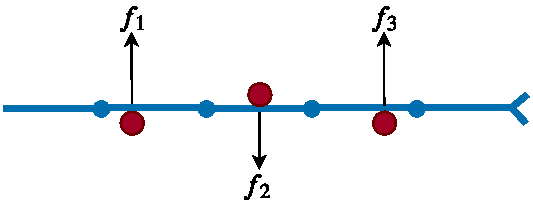
\includegraphics[width=0.6\textwidth]{figures/theory/obst-push-noprop.pdf}
    \caption{Force application yielding no propulsion}
    \label{fig:force-noprop}
\end{figure}

\begin{figure}
    \centering
    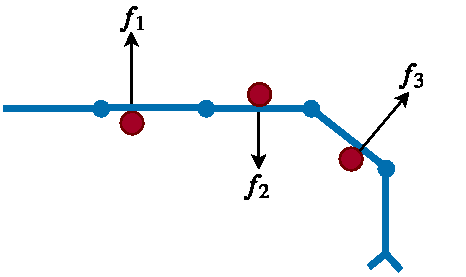
\includegraphics[width=0.5\textwidth]{figures/theory/obst-push-prop.pdf}
    \caption{Force application yielding propulsion}
    \label{fig:force-prop}
\end{figure}


The last example presenting forward propulsion does not include a desired trajectory for the snake robot to follow. Certain criteria will have to be met in the generation of the trajectory as well, and will typically be based on the composition of the snake robot. If the links are very long the snake robot will naturally not be able to shape itself along a very tightly curved path. If, on the other hand, the link length approaches zero the snake robot will resemble a natural snake and the limitations to its shape are decreased significantly. This type of robot is also referred to as a continuum robot, which according to Robinson et al. \cite{robinson1999continuum} is a continuously bending, infinite-degree-of-freedom structure. The goal in HOAL is not to adapt the snake robot composition to fit the path, but rather the path to fit the snake robot.

Figure \ref{fig:path-following} shows one case in which the curves of the desired path are sufficiently large for the snake robot to follow and one case in which the snake robot is physically unable to adjust itself perfectly to the desired path. The obstacles necessary for propulsion are left out in the illustrations.

\begin{figure}[H]
    \centering

    \subfloat[Successful path adjustment]{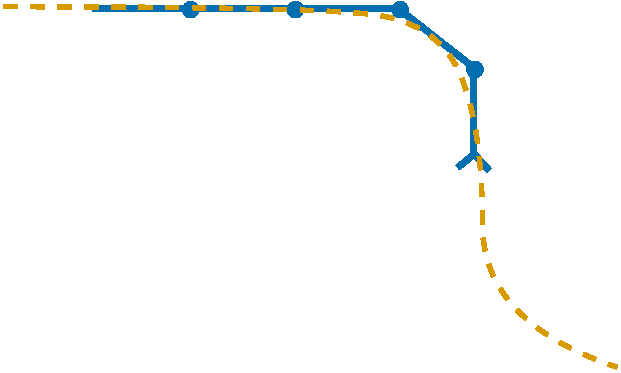
\includegraphics[width=0.5\textwidth]{figures/theory/path1.pdf}}
    \hfil
    \subfloat[Unsuccessful path adjustment]{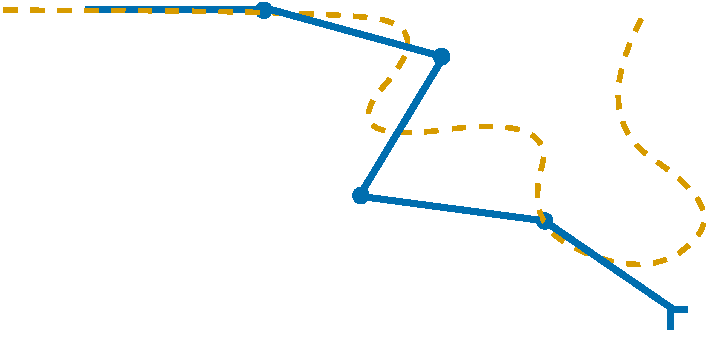
\includegraphics[width=0.5\textwidth]{figures/theory/path2.pdf}}

    \caption{Snake robot desired path following}
    \label{fig:path-following}
\end{figure}

It is clear that a distinct set of conditions for the desired path should be determined before the path planner is implemented. One hypothesis suggested by Stavdahl \cite{StavdahlNote} is that if the path consists of straight lines and circle segments, the radius of the circle segments have to be at least the same length as the snake robot link.